%\usepackage[disable]{todonotes} %<-- For when we submit

%\title{Weaving Parallel Threads}
%\subtitle{Searching for Useful Parallelism in Functional Programs}
%\author{Jos\'{e} Manuel Calder\'{o}n Trilla\inst{1} \and Simon Poulding\inst{2} \and Colin Runciman\inst{1}}
%
%\institute{University of York, York, UK \and Blekinge Institute of Technology, Karlskrona, Sweden}
%
%\begin{document}
%\maketitle
%
%\begin{abstract}
%As the speed of processors is starting to plateau, chip manufacturers are
instead looking to multi-core architectures for increased performance. The
ubiquity of multi-core hardware has made parallelism an important tool in
writing performant programs. Unfortunately, parallel programming is still
considered an advanced technique and most programs are written as sequential
programs.

We propose that we lift this burden from the programmer and allow the compiler
to automatically determine which parts of a program can be executed in
parallel. Historically, most attempts at auto-parallelism depended on static
analysis alone. While static analysis is often able to find \emph{safe}
parallelism, it is difficult to determine \emph{worthwhile} parallelism. This
is known as the \emph{granularity problem}. Our work shows that we can use
static analysis \emph{in conjunction with} search techniques by having the
compiler execute the program and then alter the amount of parallelism based on
execution speed.  We do this by annotating the program with parallel annotations
and using search to determine which annotations to enable.

This allows the static analysis to find the safe parallelism and shift the
burden of finding worthwhile parallelism to search. Our results show that by
searching over the possible parallel settings we can achieve better performance
than static analysis alone.

%\end{abstract}

\section{Introduction}
\label{sec:Intro}
The rest of this chapter describes our technique in more detail. Section
\ref{sec:blind-ParFunc} discuss the main background to this work: implicit
parallelism in functional languages. Section~\ref{sec:blind-Overview} provides
a worked example to illustrate the static analysis we perform to determine
potential parallelism.  We describe our empirical method and results in Section
\ref{sec:blind-Results}. Lastly, we offer our conclusions and discuss related
work in Section \ref{sec:blind-Conclusion}.


\section{Implicit Parallelism in Functional Languages}
\label{sec:ParFunc}
In this section we will motivate and discuss the benefits and drawbacks of
implicit parallelism in a lazy purely functional language. We will also give
a high-level overview of \emph{strictness analysis} which allows us to find safe
parallelism in lazy languages.

\subsection{Background}

Research into parallelism in lazy purely functional languages has a long
history that dates back to the early work on lazy functional languages
\citep{hughes:thesis, vGMachine, dutchBook, SPJ:PIFPL}\footnote{For a
comprehensive review we suggest \citep{hammond2000research}}. Non-strictness
makes it difficult to reason about when expressions are evaluated. This forces
the programmer to avoid the use of arbitrary side-effects. The resulting purity
means that functions in pure functional languages are \emph{referentially
transparent}, or the result of a function depends only on the values of its
arguments (i.e.  there is no global state that could effect the result of the
function or be manipulated by the function).

Purity alone is of huge benefit when dealing with parallelism. Because
functions do not rely on anything but their arguments the only communication
between threads necessary is the result of the thread's computation, which is
shared via the program's graph using the same mechanism used to implement
laziness \citep{SPJ:PIFPL}.

Laziness, while forcing the programmer to be pure (which is a boon to
parallelism), is an inherently sequential evaluation strategy. Lazy evaluation
only evaluates expressions when they are \emph{needed}. This is what allows for
the use of infinite data structures, only what is needed will be computed.

The two reductions of $sqr$ in Figure \ref{fig:eagerandlazy} illustrate the key
differences between lazy evaluation and eager, or strict, evaluation


\begin{figure}[!h]
\centering
\begin{multicols}{2}
\noindent
\begin{align*}
     \noalign{$\text{\underline{Eager Evaluation}}$}
     &sqr\ (5*5) \\
  =\ &sqr\ 25 \\
  =\ &let\ x\ =\ 25\ in\ x * x \\
  =\ &25 * 25 \\
  =\ &625
\end{align*}
\begin{align*}
     \noalign{$\text{\underline{Lazy Evaluation}}$}
     &sqr\ (5*5) \\
  =\ &let\ x\ =\ 5*5\ in\ x * x \\
  =\ &let\ x\ =\ 25\ in\ x * x \\
  =\ &25 * 25 \\
  =\ &625
\end{align*}
\end{multicols}
\caption{Eager and Lazy evaluation order for squaring a value.}
\label{fig:eagerandlazy}
\end{figure}

In the case of eager evaluation the argument to $sqr$ is evaluated
\emph{before} entering the function body. For lazy evaluation the argument is
passed as a suspended computation that is only \emph{forced} when the value is
needed (in this case when $x$ is needed in order to multiply $x*x$). Notice
that under lazy evaluation $5*5$ is only evaluated once, even though it is
used twice in the function. This is due to the \emph{sharing} of the result.
This is why laziness is often described as call-by-need \emph{with sharing}
\citep{hammond2000research}.

\medskip

In the case of $sqr$ in Figure \ref{fig:eagerandlazy}, both eager and lazy
evaluation required the same number of \emph{reductions} to compute the final
result. This is not always the case; take the following function definitions
\begin{align*}
    &bot \ :: \ Int\ \rightarrow\ Int \\
    &bot\ x\ =\ x + bot \\
    \quad & \\
    &const\ :: \ a\ \rightarrow\ b\ \rightarrow\ a \\
    &const\ x\ y\ =\ x
\end{align*}
\label{fig:botAndConst}

In an eager language the expression $const\ 5\ bot$ will never terminate,
while it would return $5$ in a lazy language as only the first argument
to $const$ is actually \emph{needed} in its body.

\medskip


This tension between the call-by-need convention of laziness with parallelism's
desire to evaluate expressions \emph{before} they are needed is well known
\citep{tremblay1995impact}. The most succesful method of combating this tension
is through the use of \emph{strictness analysis} \citep{mycroft1980theory,
wadler1987projections, hinze1995projection}.




\section{Overview}
\label{sec:Overview}
As the majority of our work is in the form of a compiler it is important to
understand its organisation. Most of the phases present in our compiler can be
found in most standard compilers for lazy functional languages with the
exception being that our compiler `iterates' by running the program and
altering the compilation based on that feedback. The compiler is organised into
8 main phases, as follow:

\begin{enumerate}
    \item Parsing
    \item Defunctionalisation
    \item Projection-based Strictness Analysis
    \item Generation of strategies
    \item Placement of \verb-par- annotations
    \item $G$-Code Generation
    \item Execution
    \item Feedback and iteration
\end{enumerate}

Parsing is completely standard and we will therefore omit discussing that stage
of compilation. An interested reader is pointed towards ``Implementing
Functional Languages: A Tutorial'' \citep{PeytonJones:IFL}.


The rest of this dissertation focuses on the static analysis phases of the
compiler (defunctionalisation, strictness analysis, and the generation of
strategies) and the feedback and iteration phase. To see how the pieces
all fit together we will demonstrate the important stages of the compiler
with two small programs.

\subsection{Automatic Parallelisation: 1990's Style}

When research into implicit parallelism was at its height in the late 1980's and 1990's
much of the focus was on using static analysis to introduce parallelism to programs.
We can see how this was done with a simple example.

The program listed in Figure \ref{fig:tak} is the Tak program benchmark, often used
for testing the performance of recursion in interpreters and code generated by
compilers \citep{ExamplesOfRecursion}.

\begin{figure}
  \input{Blind/TakPhases/Tak.hs}
\caption{Source listing for Tak}
\label{fig:tak}
\end{figure}

Luckily, this program is already first-order, so we do not need to worry
about defunctionalisation. We therefore proceed directly to our strictness
analysis. This phase of the compiler is able to determine which function
arguments are \emph{definitely} needed by each function. In the case of
\verb|tak| the strictness analysis determines that all three arguments
are needed. \todoinline{show the strictness information}

After we perform our projection-based strictness analysis we can introduce the
safe \verb-par- annotations, transforming the program into a parallelised
version. The result of this transformation on Tak is listed in Figure
\ref{fig:takParred}.

\begin{figure}[b]
  \input{Blind/TakPhases/TakParred.hs}
\caption{Source listing for Tak after analysis, transformation, and \texttt{par} placement}
\label{fig:takParred}
\end{figure}

Each needed \todo{should I define strict before this and use strict instead of
needed?} argument is given a name via a \verb-let- binding. This is so that any
parallel, or \verb-seq-ed, evaluation can be shared between threads. When there
are multiple strict arguments (as is the case for \verb-tak-) we spark the
arguments in left-to-right order except for the last strict argument, which we
\verb-seq-. This is a common technique that is used to avoid potential
collisions \citep{strategies}. Collisions occur when a thread requires the
result of another thread before that result has been evaluated. By ensuring that
one of the arguments is evaluated in the current thread (by using \texttt{seq})
we give the paralell threads more time to evaluate their arguments, lessening
the frequency of collisions.

Now that the parallelism has been introduced we can run our program on a multi-processor
machine and hope to get speedups.

\todoinline{Show results of sequential vs. parallel tak}

This is the hallmark of the conventional approach to automatic parallelism:
determine a method of identifying potential parallelism, then transform the
program to exploit that parallelism. However, this approach only addresses one
half of the criteria needed for taking advantage of implicit parallelism: where
is parallelism \emph{safe}?

While static analysis has determined that \verb-x'- and \verb-y'- can be
evaluated in parallel \emph{safely}, it does not determine whether parallel
evaluation of those expressions is \emph{worthwhile}. This is the crux of the
\emph{granularity problem}. In the case of Tak we can run the program and see
that we do indeed achieve performance increases from the parallelism that was
introduced\footnote{But it is not the fastest that we can achieve!} \todo{show
with charts!}. However, there is no process by which the compiler may alter its
decision of what \verb|par| annotations to introduce.

In the literature it was common to use further static analysis to estimate the
cost of evaluating an expression. This estimate would then be used to avoid
introducing parallelism that is too \emph{fine-grained}. This was commonly done
with both heuristic oracles and/or using a static cost analysis
\citep{hogen1992automatic} \tocite{A cost analysis paper}.

% TODO: find a place for this, a discussion of collisions would be good.
%This is best explained through a simple example:
%
%\begin{figure}
%\begin{center}
%\begin{BVerbatim}
%fib :: Int -> Int
%fib 0 = 0
%fib 1 = 1
%fib n = let x = fib (n - 1)
%            y = fib (n - 2)
%        in par x (seq y (x + y))
%\end{BVerbatim}
%\end{center}
%\end{figure}
%
%There are two threads interacting during the execution of \verb-fib-: The
%current thread of execution, $P$ (for parent), and the thread sparked by
%\verb-par x-, $C$ (for child). If the \verb-seq- were a \verb-par-, or absent
%entirely, in \verb-fib- then there is the possibility that $P$ would require
%\verb-x- immediately when evaluating \verb-x + y-. This would cause $P$ to
%block on $C$, awaiting the completion of \verb-x-'s evaluation. By having the
%function use \verb-seq- we ensure that productive work was accomplished even if
%$P$ needs to wait for $C$'s completion.
%
%\hfill$\Box$

%The function \verb-tak- happens to be strict in all three of its arguments.
%Therefore we lift all three arguments into a \verb-let- binding, allowing their
%results to be shared. Then we arrange the parallel evaluation of each of the
%arguments using \verb-par- and \verb-seq- annotations. The \verb-seq-
%annotation is to ensure that \verb-z'- is evaluated in the current thread, so
%that the current thread does not immediately block waiting for \verb-x'- or
%\verb-y'-.
%


\subsection{Static Analysis is Not Enough}

The propensity for researchers to prefer static analysis over dynamic technique
has many benefits, particularly the fact that they incur no runtime costs and
have many decades of work to build upon. However, in some cases the
(over)reliance on static analyses can be a hindrance instead of a benefit. We
argue that implicit parallelism is an area that requires compiler writers to
abandon the `static analysis only' methodology.

An intuitive argument for our view is that parallelising programs is something
that even \emph{experts} have difficulty with. The work of determining what
parallelism is worthwhile is often an \emph{iterative} process between the
programmer and the program. In other words; programmers do not `write once',
but instead annotate a program, profile the program, and alter the program
according to the results of profiling. Why do we forbid compilers from utilising
the same process?

Program analysis does not have to pick sides; compilers can benefit (if the
implementors wish) from \emph{both} static and dynamic analysis. In the
case of implicit parallelism this means having the compiler perform a form of
static analysis that provides an initial decision about parallelism in the
program, then having those decisions either confirmed or rejected by dynamic,
profile-driven analysis. There are several ways to achieve this goal. The
method we suggest is to utilise \emph{feedback-directed}
compilation\footnote{Sometimes referred to as feedback-directed optimisation or
iterative compilation}.

\defineword{Feedback-Directed Compilation}{The use of runtime profiles from
previous executions of the program in order to inform an aspect of compilation
or optimisation.}

This frees the compiler from having to answer all of the difficult questions
statically (and in one shot). Might and Prabhu suggest that the compiler has
two question it must ask when parallelising a sequential program \tocite{Might's stack reachability}:

\begin{enumerate}
    \item Where is parallelisation \emph{safe}?
    \item Where is parallelisation beneficial?
\end{enumerate}

Compiler writers have many tools available when wanting to answer the first:
strictness analysis, dependency analysis, control-flow analysis, etc.
\citep{hogen1992automatic, might2009interprocedural}. In fact, these analyses
are very good at answering the first question. The issue that has plagued work
in automatic parallelisation is that there is often \emph{too much} safe
parallelism\footnote{This is true for pure languages, in languages that allow
arbitrary side-effects finding safe parallelism can be more difficult.}.
Determining the answer to the second question then becomes essential.
Unfortunately determining the cost (or benefit) of evaluating an
expression in parallel is notoriously difficult to do statically
\citep{hogen1992automatic, might2009interprocedural}.


The problem is that while the safety of parallelising an expression is a static
property of the program, the benefit is also affected by extrinsic factors such
as the architecture the program is executed on. To be more precise; if there is
a minimum cost to create parallelism, static analysis can determine that some
expressions are definitely \emph{not} worthwhile (by approximating the cost of
evaluating an expression `upwards'), however, static analysis cannot determine
that an expression is \emph{definitely} worthwhile. This is because the benefit
of parallelising an expression is a function of \emph{more} than the static
semantics of a program.

Let us consider a simple thought experiment:

First, consider an ideal parallel machine that has an infinite number of
processing units, zero-cost communication, and no context switches (each task
gets its own processor)\footnote{We did say \emph{ideal} machine.}. The only
cost to creating parallelism is the exact cost of the machine instructions used
to initialise the parallel task. If a task requires less time than the
initialisation cost, it is a net cost to the program and not worthwhile for
parallelism. While unrealistic, this scenario demonstrates that there are some
expressions that will not be worthwhile no matter the final program substrate
\todo{substrate?}.

Now consider the same machine, except with a finite number of processing units.
Because each task is no longer able to retain a processor to itself, the machine
must schedule tasks which imposes a context-switch cost on the tasks that
are interrupted. Now whether a task is worthwhile depends not only on its
intrinsic cost, but on the effect it has on the rest of the computation by
interrupting other tasks. It is easy to see that more context-switches occur
as the number of processing units available is reduced.

The difficulty of predicting the benefit of a parallel task becomes even more
difficult as the machine becomes more realistic. Because of this we feel that
it is sensible to ask: ``Why have the compiler try at all?''. Instead of
having the compiler approximate this complex program property, we can run
the program itself and have the compiler `see' the effect its parallelisation
has on the final program.

One question remains: in what way do we combine the static analysis with the
feedback-directed compilation? There are several apparent approaches:

\begin{enumerate}
    \item Have the compiler introduce parallelism sparsely, and use the
        iteration to introduce more parallelism
    \item Have the compiler introduce what seems to be \emph{too much}
        parallelism and have the iteration remove some of the parallelism
    \item Have the compiler provide an initial `reasonable' parallelisation
        and have the iteration introduce/remove parallelism as necessary
\end{enumerate}

In choosing our approach we chose to play to the strengths of the language we
are conducting our experiments with. In pure functional languages there is an
abundance of safe parallelism. Historically, parallelism in pure lazy languages
often suffers more from the granularity problem than from a lack of available
parallelism \tocite{someone}. For this reason we have opted to use the second
approach: use static analysis to introduce as much parallelism as possible and
use runtime feedback to disable some of the introduced parallelism.

We note that for a language that allows arbitrary side-effects it may be more
beneficial to use the first approach as the runtime feedback would aid in
determining which tasks were actually independent.

Later in Chapter \ref{chap:future} we will explore a variant of the third
approach.

\subsection{Automatic Parallelism in the 21st Century}

In order to address this issue we take advantage of
two key properties of our \verb-par- annotations:

\begin{enumerate}
    \item Each introduced \verb-par- sparks off a unique subexpression
            in the program's source
    \item The semantics of \verb-par- (as shown in Figure \ref{fig:seqandpar})
            allow us to return its second argument, ignoring the first,
            without changing the semantics of the program as a whole
\end{enumerate}

These two properties allow us to represent the \verb-par-s placed by static
analysis and transformation as a bit string. Each bit represents a specific
\verb-par- in the program's AST. When a \verb-par-'s bit is `on' the \verb-par-
behaves as normal, sparking off its first argument to be evaluated in parallel
and return its second argument. When the bit is `off' the \verb-par- returns
its second argument, ignoring the first.

This allows us to change the \emph{operational} behaviour of the program without
altering any of the program's semantics. In other words, we are able to \emph{try}
evaluating subexpressions in parallel, without the risk of introducing behavior
that was not present in the original program.

% Below this is the overview from the IIP paper
% TODO: Merge overviews!
%\todo[inline]{Merge this overview with other overview}
%
%In this section we present the overall picture of our technique. Much of the
%discussion will center around the code presented in Figure \ref{sumLast}. In
%order to understand the code, it is useful to understand the architecture of the
%compiler.
%
%\todoinline{Canibalise some of the following for the overview above. Some of
%the content is good but it needs to be integrated with the above, right now
%it's just repetition with a few new things (how to read the code, introduce
%defunctionalisation, etc.)}

%\subsection{A Program Before Iteration}
%
%%\begin{figure}[t!]
%%  \input{Informed/SumPhases/SumEulerProcessed.core}
%%\caption{Core representation of \texttt{SumEuler} after defunctionalisation, demand
%%         analysis, and the introduction of initial \texttt{par} sites along
%%         with their associated strategies.(Auto-generated names have been
%%         replaced for better readability)}
%%\label{sumLast}
%%\end{figure}
%
%The code listed in Figure \ref{sumLast} is the resulting core representation
%of the program in Figure \ref{sumOrig} after our analysis and transformations.
%Specifically, the program has passed through compiler stages 1-5.
%
%Before we dive into the program itself, note the following points:
%
%\begin{itemize}
%    \item We only present the functions that have changed as a result of transformation
%    \item We have replaced auto-generated names with easier to read names
%    \item Functions ending in `S$N$' are derived strategies
%    \item Functions with an underscore in the name are the result of defunctionalisation
%\end{itemize}
%
%Taking a look at the program we can see several of the core ideas.
%
%\paragraph{Defunctionalisation}
%The application of \verb-map- to \verb-euler- has been replaced by a call to
%the specialised \verb-map_euler- function.  We no longer have the functions
%\verb-map- or \verb-filter- instead we have specialised versions of these
%functions (e.g. \verb-map_euler-)
%
%\paragraph{Introduction of parallelism}
%Two calls to \verb-par- have been introduced in the \texttt{main} function. Our
%work uses the traditional style for the parallel combinator \citep{strategies}
%
%\begin{verbatim}
%    par :: a -> b -> b
%    par x y = y
%\end{verbatim}
%
%The first argument is \emph{sparked} off to be evaluated in parallel and the
%function returns the second argument. This style is what allows us to easily
%\emph{switch off} a particular \verb-par- which causes that switched off
%\verb-par- to act like \verb-flip const-. This is explored further in
%\S\ref{sec:switchPar}.
%
%Each application of \verb-par- introduced by our compiler takes the following
%form: \verb-par (s x) e- where \verb-(s x)- is the application of derived
%strategy \verb-s- to a variable \verb$x$ and \verb$e$ is an expression containing \verb$x$ as a
%free variable.  In a \emph{top-level definition} like \verb-main-, \verb$x$ will be a
%name introduced by a \verb-let- expression. For \verb-par-s within the
%strategies themselves, \verb$x$ will be a name introduced by case analysis.
%
%\paragraph{Demand Analysis and Strategies}
%
%The compiler has introduced a number of strategies into the program. These
%strategies are derived based on the results of a demand analysis. A simple
%example from the program is the transformed version of \verb-length-. Because
%\verb-+- (for non-lazy integers) requires both arguments to be fully evaluated, it is safe to 
%evaluate the arguments to \verb-+- in parallel to the execution of its body.
%In order to benefit from the parallel evaluation, the structure must be shared.
%The introduction of the name \verb-len- accomplishes this. Because the type
%of \verb-len- is \verb-Int- evaluating the expression to WHNF is sufficient to
%evaluate the value fully. 
%
%Looking at the body of \verb-euler- where \verb-length- is called we see a
%similar pattern. In this case the demand analysis determines that it is
%safe the evaluate the \emph{spine} of the list passed to \verb-length-.
%The expression is given the name \verb-ys- and the strategy \verb-eulerListS1-
%is derived based on this information. Notice that the elements of the list
%passed to \verb-eulerListS1- are ignored in its body. 
%
%There are cases where there is a strict demand on an expression but we
%do not introduce parallel evaluation of the expression. This can be seen
%in the first argument to \verb-+- in the body of \verb-length-. The rules
%for which subexpressions are considered \emph{definitely} not worthwhile
%are discussed in \S\ref{sec:introPar}.

\paragraph{Iterative Improvement}

Just because an expression is \emph{able} to be evaluated in parallel does not
mean that doing so is beneficial. This is one of the critical problems in
implicit parallelism \citep{hogen1992automatic, hammond2000research,
Jones2009Tuning}. To combat this we run the program as presented in Figure
\ref{fig:takParred} and collect statistics about the amount of productive work
each \verb-par- is responsible for. The \verb-par-s that do not introduce a
worthwhile amount of parallelism are disabled, freeing the program from
incurring the overhead of managing threads for tasks with insufficient
granularity\footnote{This can be seen as a more extreme variation of Clack and
Peyton Jones' ``Evaluate and die!'' model of parallelism \citep{clack1986four}:
Evaluate \emph{a lot} or die!}.

Luckily, the \verb-Tak- program has so few \verb-par-s that an exhaustive
exploration of the possible settings is easy. Table \ref{tab:takSettings}
shows the resulting speedup (as compared to the program with all parallelism
turned off) from the different possible \verb-par- settings. The bitstring
``$10$'' represents the version of \verb-Tak- where the \verb-par- labelled
$0$ in \ref{fig:takParred} is on and the \verb-par- labelled $1$ is off.

\begin{table}[h!]
\centering
\caption{Performance of \texttt{Tak} with different \texttt{par} settings}
\vspace{10pt}
\begin{tabular}{c || c c c c}
    \       & 00 & 01   & 10   & 11 \\
    \hline
    speedup & 1  & 1.56 & 0.43 & 0.97
\end{tabular}    
\label{tab:takSettings}
\end{table}

As we can see, more \verb-par-s is not necessarily better. In fact, for our
interpreter the setting $10$ results in quite a lot of thread collisions,
meaning that a thread pays the overhead for its paralellism and is almost
immediately blocked.  Paying the cost of creating and managing the parallelism,
but not being able to perform an actual work is why the program performs
\emph{worse} than the version of \verb-Tak- with all the parallelism switched
off.

So why introduce this parallelism in the first place? Because the granularity
and possible interference of parallel threads is difficult to know
\emph{statically} at compile time. Not only is it difficult to know these
properties statically, but these properties differ from architecture to
architecture \citep{SteuwerPortable}. If we err on the side of generosity with
our \verb-par- annotations we can then use \emph{runtime} profiling to gather
information about the granularity and interference of threads. 


\section{Summary}

This chapter provided a high-level overview of our technique for exploiting the
parallelism that is inherent in functional programs. We motivated our choice of
a \emph{lazy} language (normal-order reduction using call-by-need) by
considering its emphasis on purity and the fact that the sharing of values is
built-in to the evaluation model.

We introduced the structure of our compiler and walked through the steps of our
technique using the \verb-Tak- program as a small example. This allows for a
clearer notion of where the remaining chapters fit into our technique and
provides a common vocabulary for the rest of the thesis.

\paragraph{}

Now that we have presented the high-level view of our work we will now explore
each of the stages in depth. Chapter \ref{chap:discovery} introduces strictness
analysis and discusses the history of its development and why we have chosen
\emph{projection-based} strictness analysis for our compiler. Chapter
\ref{chap:derivation} presents how to use the results from projection-based
strictness analysis to \emph{automatically} derive parallel strategies that are
then used to introduce parallelism into the source program. Chapters \ref{chap:blind}
and \ref{chap:prof-search} represent the iterative phase of our compiler, discussing
two methods of searching the space of \verb-par- settings.


% \section{Iterative Improvement}
% \label{sec:IterativeImprovement}
% Now we have the machinery in place to \emph{improve} the initial placement
of parallel annotations by repeatedly running the program but altering
the bit string that represents the parallel annotations in the program.

%\paragraph{Compiler Pipeline} Figure \ref{fig:pipeline} shows the pipeline of
%our compiler \footnote{Lexing and parsing are omitted as they are done in
%the standard way and will not be discussed in this paper}. Each of the phases
%of the compiler is designed to facilitate the loop at the end of the pipeline.
%This feedback loop between the program runtime and the \verb-par- switching is
%the basis of our technique and the cornerstone of our contribution.
%
%\begin{figure}[t]
%\includegraphics[scale=0.5]{Blind/Figures/pipeline4.eps}
%\caption{Architecture of the Auto-Parallelising Compiler}
%\label{fig:pipeline}
%\end{figure}


\section{Experimental Setup and Results}
\label{sec:Results}
In this section we evaluate the use of search in finding an effective enabling
of \verb-par-s that achieves a worthwhile speed-up when the parellelised
program is run in a multi-core architecture.  As a reminder, the starting point
for our proposed technique is a program that was originally written to be run
sequentially on a single core; static analysis identifies potential sites at
which \verb-par- functions \emph{could} be applied; and then search is used to
determine the subset of sites at which the \verb-par- is actually used.

% The evaluation is motivated by an intended use-case for the technique: that
% an effective---not necessary optimal---placement of \verb-par-s can be found
% during the equivalent of a coffee break.

\subsection{Method}

The following four algorithm configurations were evaluated:
\begin{itemize}
	\item hill-climbing with all-on initialisation
	\item greedy with all-on initialisation
	\item hill-climbing with random initialisation
	\item greedy with random initialisation
\end{itemize}

Each algorithm configuration was evaluated for four settings of the number
cores: 4, 8, 16 and 24 cores. Each algorithm / core count combination was
evaluated against each of the seven benchmark programs described above.

Since both search algorithms are stochastic, multiple runs were made for each
algorithm / core count / benchmark combination, each using 30 different
seeds\footnote{All seeds were obtained from \url{www.random.org}.} for the
pseudo-random number generator.  For all runs, after each fitness evaluation,
the best bit string found and its fitness (the number of reductions made by the
main thread), was recorded.

In addition, the fitness (number of reductions) was evaluated for a bit string
where all bits are set to 1: this equivalent to using the static analysis
without optimisation using search.  This evaluation was made for each
combination of core count and benchmark.  Finally, the fitness was evaluated for the
sequential version of each benchmark.

\paragraph{Overheads} Our runtime system allows us to set the cost of creating
a parallel task, this models the overhead present in real systems. Using the
Criterion \citep{criterion} benchmarking library we found an approximate cost
for the creation of a \verb|par| in GHC's runtime\footnote{The code for
benchmarking the cost of a \texttt{par} is available at
\url{https://github.com/jmct/par-experiments}}. For the experiments we have
chosen an overhead of $300$ reductions for each call to \verb|par|.

\subsection{Results}

The results are summarised in Table \ref{tab:speedups}.  This table compares
the speed-up, calculated as the ratio of the medians of the reduction counts,
of hill-climbing with all-on initialisation compared to (a) the parallelisation
that would result from the static analysis without optimisation; (b) the
sequential version of the program; (c) the greedy algorithm with all-on
initialisation; and (d) the hill-climbing algorithm with random initialisation.
The speed-up is calculated as the factor by which the number of reductions is
reduced, and so values greater than 1 indicate that the program parallelised
using hill-climbing with all-on initialisation would be faster in the
multi-core environment.  Values in bold in the table indicate that differences
between the algorithms used to calculate the speed-up are statistically
significant at the 5\% level using a one- or two-sample Wilcoxon test as
appropriate\footnote{Since in the following we discuss the results for each
benchmark program, or combination of benchmark program and number of cores,
individually as well as for the entire set of results as a family, we do not
apply a Bonferroni or similar correction to the significance level.
Nevertheless we note here that most of the currently significant differences
would remain significant if such a correction were applied.}. The values in
blue are both statistically significant at the 5\% level \emph{and} exhibit a
speedup for more than 5\%. This separates the statistically significant
speedups that are unlikely to manifest on a real machine. The results for
\verb|Taut|, for example, are statistically faster, but the difference is so
minute (less than one tenth of a percent in all cases!) that the
non-determinism of a real architecture is likely to render the speedup
irrelevant.

\begin{table}
\caption[Results from using heuristic search]{The speed-up, calculated as the ratio of the medians of the reduction counts, achieved by the hill-climbing algorithm using all-on initialisation.}
\smallskip
\smallskip
\centering
	\sisetup{detect-weight=true, detect-inline-weight=math,round-mode=figures, round-precision=4}
\begin{tabular}{c c S S S S}
 	      & & \multicolumn{4}{c}{hill-climbing search speed-up compared to:} \\[0.25cm]
 SUT      & {Cores} & {\parbox{2cm}{\centering Static Parallel}} & {\parbox{2cm}{\centering Sequential}} & {\parbox{2cm}{\centering Greedy}} & {\parbox{2cm}{\centering Random Init}} \\[0.25cm] \hline
\multirow{4}{*}{MatMul}    & 4 & \bfseries\color{blue} 4.90301661707919  & \bfseries\color{blue} 1.02124759973798  &  1  &  1  \\
    & 8 & \bfseries\color{blue} 4.62464276508472  & \bfseries\color{blue} 1.02124759973798  &  1  &  1  \\
    & 16 & \bfseries\color{blue} 4.48549626511679  & \bfseries\color{blue} 1.02124759973798  &  1  &  1  \\
    & 24 & \bfseries\color{blue} 4.43914308383459  & \bfseries\color{blue} 1.02124759973798  &  1  &  1  \\
\hline
\multirow{4}{*}{Queens}    & 4 & \bfseries\color{blue} 1.08002338656061  & \bfseries\color{blue} 1.29449651880535  &  1  &  1  \\
    & 8 & \bfseries 1.04284123826334  & \bfseries\color{blue} 1.36903090592333  &  1  &  1  \\
    & 16 & \bfseries 1.01658424583816  & \bfseries\color{blue} 1.40075887342919  &  1  &  1  \\
    & 24 & \bfseries 1.00284839597168  & \bfseries\color{blue} 1.40077452594306  & \bfseries 1.000005587155  &  1  \\
\hline
\multirow{4}{*}{Queens2}   & 4 & \bfseries\color{blue} 6.47871841266272  & \bfseries\color{blue} 3.84268026498045  &  1  &  1  \\
    & 8 & \bfseries\color{blue} 6.4214444887208  & \bfseries\color{blue} 7.60677419801831  &  1  &  1  \\
    & 16 & \bfseries\color{blue} 6.26286318030988  & \bfseries\color{blue} 14.7914211715831  &  1  &  1  \\
    & 24 & \bfseries\color{blue} 6.10111087862129  & \bfseries\color{blue} 21.5370475166917  &  1  &  1  \\
\hline
\multirow{4}{*}{SodaCount} & 4 & \bfseries\color{blue} 4.23709552156544  & \bfseries\color{blue} 3.77256127760359  & \bfseries 1.00090381935946  & \bfseries\color{blue} 1.05522740981559  \\
    & 8 & \bfseries\color{blue} 3.54406724309037  & \bfseries\color{blue} 6.20691010897515  & \bfseries 1.00698493625413  & \bfseries\color{blue} 1.07054373432511  \\
    & 16 & \bfseries\color{blue} 3.10964257836354  & \bfseries\color{blue} 10.3951019801297  & \bfseries\color{blue} 1.08075042082402  & \bfseries\color{blue} 1.07197550990065  \\
    & 24 & \bfseries\color{blue} 2.80981399852391  & \bfseries\color{blue} 13.2551680242675  & \bfseries 1.00369023678455  &  1  \\
\hline
\multirow{4}{*}{SumEuler}  & 4 & \bfseries\color{blue} 1.49372579894484  & \bfseries\color{blue} 3.94797162309201  &  1  &  1  \\
    & 8 & \bfseries\color{blue} 1.48574818274656  & \bfseries\color{blue} 7.77250594496659  &  1  &  1  \\
    & 16 & \bfseries\color{blue} 1.46021192398224  & \bfseries\color{blue} 14.7739589421968  & \bfseries 1  &  1  \\
    & 24 & \bfseries\color{blue} 1.43221979480656  & \bfseries\color{blue} 20.6898343519261  & \bfseries 1  &  1  \\
\hline
\multirow{4}{*}{Tak}       & 4 & \bfseries\color{blue} 1.60884879829089  & \bfseries\color{blue} 1.55987328230559  &  1  &  1  \\
    & 8 & \bfseries\color{blue} 1.60872875931022  & \bfseries\color{blue} 3.11836989833956  &  1  &  1  \\
    & 16 & \bfseries\color{blue} 1.60840817353438  & \bfseries\color{blue} 6.22950966713651  &  1  &  1  \\
    & 24 & \bfseries\color{blue} 1.607828276573  & \bfseries\color{blue} 9.32979045709963  &  1  &  1  \\
\hline
\multirow{4}{*}{Taut}      & 4 & \bfseries 1.00030996496344  & \bfseries 1.00031731386223  & \bfseries 1.0000038116695  &  1  \\
    & 8 & \bfseries 1.00026247377892  & \bfseries 1.00038387590672  & \bfseries 1.00000088436617  &  1.000  \\
    & 16 & \bfseries 1.00026848403891  & \bfseries 1.00039382131741  & \bfseries 1.00001488189584  &  1  \\
    & 24 & \bfseries 1.00026848403891  & \bfseries 1.00039382131741  & \bfseries 1.00001488189584  &  1  \\
\end{tabular}\\
\label{tab:speedups}
\end{table}

\subsection{Discussion of Research Questions}

We can now look again at our four research questions from Section
\ref{sec:hypotheses} and determine whether our experiments have given us
meaningful results to any of them.

\paragraph{RQ1}
For most of benchmarks there is a relatively large speed-up of the
hill-climbing algorithm compared to the default parallelisation where all
\verb-par-s are enabled.  The largest speed-ups are for \verb|Queens2| where we
might expect a wall-clock run time that is more than 6 times better than the
default parallelisation.  For \verb|Queens| and \verb|Taut| the speed-ups are
closer to 1, but are in all cases statistically significant.

An interesting property regarding the speedups as compared to the static
placement is that they decrease as the number of cores increases.  This aligns
with our intuition for parallel programs. As the number of cores goes up, the
static placement \emph{gets away} with non-optimal \verb|par| placement. With
more cores, there is less contention for the resources of the machine. A
\verb|par| that does more work than its overheads is less likely interrupt
another, more productive thread. When the number of cores is lower, the
contention makes even productive \verb|par|s detrimental because they interrupt
threads that are even more productive.

We conclude that both the greedy and the hill-climbing algorithm can improve
parallel performance across a range of benchmarks and across a range of core
counts when compared to using the static placement of parallelism.

\paragraph{RQ2}
For \verb|Queens2| and \verb|SumEuler|, the speed-up compared the sequential
version of these benchmarks is almost linear: it approaches the number of cores
available.  For example, for \verb|SumEuler| on 4 cores, the speed-up compared
to the sequential version is $3.95$.  A linear speed-up is the best that can be
achieved, and so these results are indicative that our proposed technique could
be very effective in practice.  Meanwhile, for other benchmarks such as
\verb|MathMaul| and \verb|Taut|, there is little speed-up over the sequential
version of the benchmark.

\paragraph{RQ3} The results show that for most benchmarks, there is little
difference in the speed-up achieved by the hill-climbing and greedy algorithm.
(For clarity, the table shows the comparison only between the two algorithms
using all-on initialisation, but similar results are obtained when
initialisation is random.) Only for \verb|SodaCount| is there a non-trivial and
statistically significant difference between the hill-climbing and greedy
algorithm for all core sizes.  Figure \ref{fig:evals} performs a further
analysis for this research question: for two of the benchmarks, it plots the
best speed-up (compared to sequential) obtained so far by the algorithm against
the number of fitness evaluations.  For \verb|Queens2| at all core counts, the
greedy algorithm finds the same best speed-up as the hill-climbing, but finds
it in fewer fitness evaluations, i.e. the search is faster.  For
\verb|SodaCount|, the greedy algorithm finds its best speed-up in relatively
few evaluations. The hill-climber takes longer but finds a better speed-up at
all cores counts; the difference is most noticeable in the results for 16
cores. For the goal of having a compiler that provides you with a faster
program while you take a tea break, the greedy algorithm seems satisfactory.
For frequently-used benchmarks that account for a significant part of a
system's performance, the additional effort required to find the best
parallelisation using hill-climbing may be justified, but will depend on
context. In the end this is a subjective trade off, we feel that the results
support the use of the greedy algorithm unless finding the optimal solution
is absolutely necessary.


\begin{figure}[H]
\centering
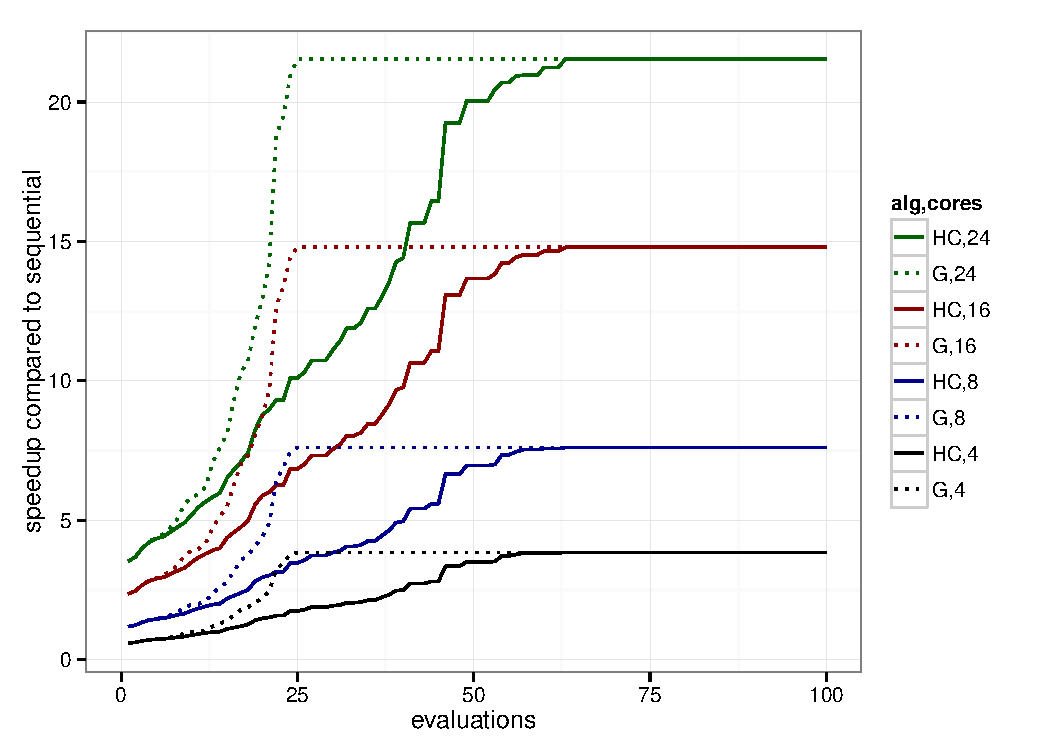
\includegraphics[scale=0.75]{Blind/Figures/speedup_by_evals_Queens2_allon_median.pdf}\\
(a) Queens2\\
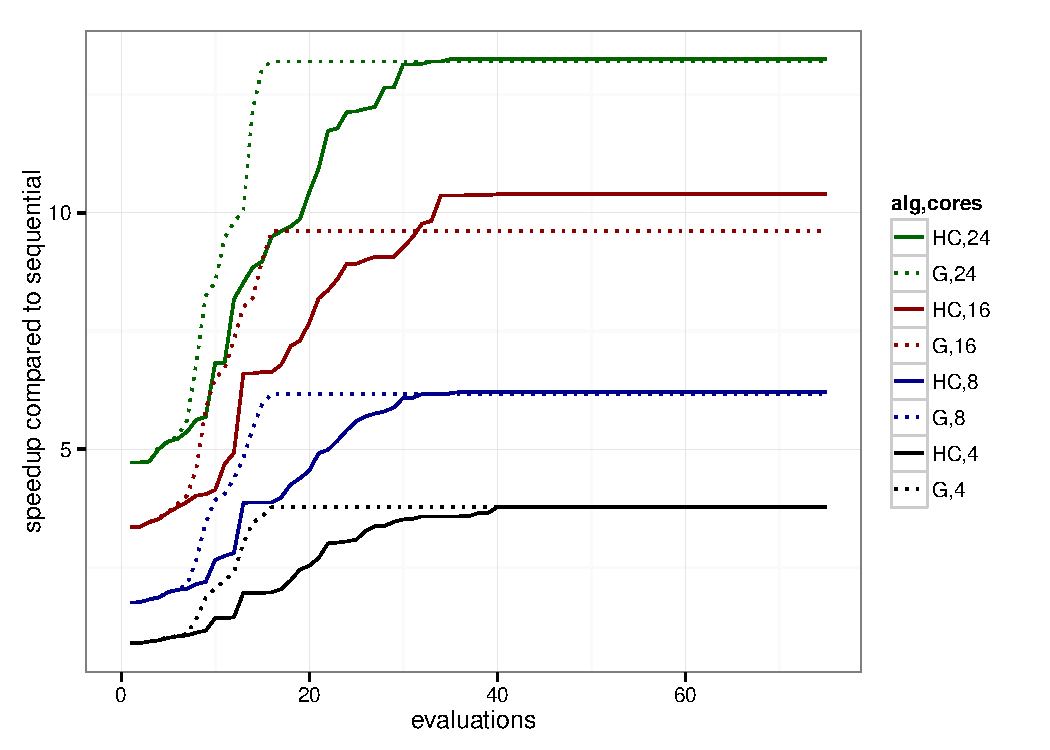
\includegraphics[scale=0.75]{Blind/Figures/speedup_by_evals_SodaCount_allon_median.pdf}\\
(b) SodaCount\\
\caption[Speedups against number of fitness evaluations for \texttt{Queens2} and \texttt{SodaCount}]{The speed-up, calculated as the ratio of the medians of the reduction counts, obtained so far by the algorithm plotted against the number of fitness evaluations. HC and G indicate the hill-climbing and greedy algorithm respectively, both using all-on initialisation. The numbers following the algorithm abbreviation indicate the number of cores.}
\label{fig:evals}
\end{figure}

\paragraph{RQ4}
For most benchmarks there is no statistically significant difference between
all-on and random initialisation.  For \verb|SodaCount|, the all-on
initialisation is slightly better for core counts of 4, 8, and 16.  This result
provides evidence that all-on initialisation may be beneficial, but requires
further investigation to confirm the generality.

\paragraph{}

The only results elided in Table \ref{tab:speedups} are the runtimes for the
greedy search with a random initialisation. This is because the random
initialisation produces inferior results in all cases and the same insight can
be gathered from studying the hill-climbing results for random initialisation.


\section{Related Work}
\label{sec:Related}
Research into parallel \emph{functional} programming has been an active research area
since the early 1980s. Before research into implicit parallelism fell out of
favor, much of the work focused on the use of static analysis alone in
parallelising programs \cite{hammond2000research, hogen1992automatic}. Harris
and Singh used runtime feedback to \emph{find} parallelism in functional
programs without the use of static analysis \cite{feedbackImplicit}. Our
approach can be seen as reversal of their approach, \emph{introduce}
parallelism at compile-time and \emph{remove} parallelism using runtime
feedback.

A number of researchers in the late 1990s applied metaheuristic search to transform serial \emph{imperative} programs into parallel ones.  Both Nisbet \cite{nisbet} and Williams \cite{williams:thesis} independently targeted FORTRAN programs using metaheuristics to find an appropriate sequence of code transformation to enable the program to take advantage of a target parallel architecture.  The Paragen framework described by Ryan and his collaborators applies genetic programming to optimise a tree-like representation of parallelising transformations that are applied to blocks of code, and a linear representation of transformations that are applied to loops in the program \cite{ryan1999automatic}.  The fitness used by Paragen is a combination of the speed-up obtained and the equivalence of the serial and parallel versions of the program based on a post hoc analysis of data dependencies.  The two key differences from the work described in this paper are that: (a) here the search does not derive a sequence of transformations, but instead determines which potential transformations, found by prior static analysis, are enabled; and, (b) any transformed parallel program is guaranteed to be equivalent to the original serial program by construction.  We believe that these differences may facilitate scalability in our approach.



\section{Conclusions}
\label{sec:Conclusion}
We feel that this chapter has provided evidence that the combination of static
analysis and search can parallelise programs more effectively than through
static analysis alone. For some programs we are able to achieve close to linear
speed-ups which is as performant as can expected. These results are promising
for those looking to add iterative capabilities to their compiler but without
the ability to adapt the runtime system. By choosing an appropriate
representation of the available parallelism in a program, we are able to use
standard search techniques to search the possible parallel configurations.

The success of the greedy algorithm was somewhat surprising. It further
supports the idea that the vast majority of potential parallelism in any given
program does not make up for the overhead costs associated with creating and
managing that parallelism.


\bibliographystyle{splncs03}
\bibliography{literature.bib}

%\appendix
%\section{Representation of Projections}
%\label{sec:Projections}
%The shortcomings of the analyses based on the abstract interpretation of
programs motivated Wadler and Hughes to propose using \emph{projections} from
domain theory to analyse strictness \citep{wadler1987projections}.

For our purposes projection-based analysis provides two benefits over abstract
interpretation: the ability to analyse functions over arbitrary structures, and
a correspondence with parallel strategies \citep{marlow2010seq, strategies}.
This allows us to use the projections provided by our analysis to produce an
appropriate function to compute the strict arguments in parallel.

We can frame the differences in the two approaches by thinking about what each
analysis is answering. Strictness analysis by abstract interpretation asks
``When passing $\bot$ as an argument is the result of the function call
$\bot$?''. Projection-based strictness analysis instead asks ``If there is a
certain degree of demand on the result of this function, what degree of demand
is there on its arguments?''.

What is meant by `demand'? As an example, the function \verb'length' requires
that the input list be finite, but no more. We can therefore say that
\verb'length' \emph{demands} the spine of the argument list. The function
\verb'append' is a more interesting example:

\begin{alltt}
        append :: [a] -> [a] -> [a]
        append []     ys = ys
        append (x:xs) ys = x : append xs ys
\end{alltt}

As mentioned in the previous section the first argument must be defined to the
first cons, but we cannot know whether the second argument is ever needed.
However, what if the \emph{result} of \verb'append' needs to be a finite list?
For example:

\begin{alltt}
    lengthOfBoth :: [a] -> [a] -> Int
    lengthOfBoth xs ys = length (append xs ys)
\end{alltt}

In this case \emph{both} arguments to \verb'append' must be finite. Projections
can be used to formalise this type of context \citep{wadler1987projections,
hinze1995projection}, which we call a \emph{demand context}.

\defineword{Demand Context}
           {The depth of a structure that is needed by the consumer of a
            function's result.}

Demand Contexts allow us to reason about the \emph{use} of a function's result,
letting us reason about functions like \<append\> more accurately. This, combined
with their ability to analyse functions of arbitrary types without the need to
design abstract domains by hand make projection-based analysis the most
realistic for our purposes of utilising implicit parallelism.

\pagebreak

\subsection{Semantics of Projections}

Given a domain $D$, a projection on $D$ is a continuous function
$\pi \ : \ D \rightarrow D$ that satisfies

\begin{align}
\pi \sqsubseteq ID \\
\pi \circ \pi = \pi
\end{align}

Equation (3) ensures that a projection can not add any information to a value,
i.e. all projections approximate the identity function. Idempotence (4) ensures
that projecting the same demand twice on a value has no additional effect. This
aligns with our intuition of demand. If we demand that a list is spine-strict,
demanding spine-strictness again does not change the demand on the list.

Because we want the introduction of parallelism to be semantics-preserving we
use the following safety condition for projections:

\begin{equation}
\gamma \ \circ \ f = \gamma \ \circ \ f \ \circ \ \pi
\end{equation}

Given a function $f \ : X \rightarrow Y$, and demand $\gamma$ on the
\emph{result} of $f$, projection-based analysis propagates the demand given by
$\gamma$ to the arguments of $f$. This results in the demand on the
\emph{arguments} of $f$ given by $\pi$.  The analysis aims to find the
\emph{smallest} $\pi$ for each $\gamma$, but approximating towards $ID$ (as
it is always safe to project the identity).

\paragraph{Demands on Primitives}
On unlifted base types, such as unboxed integers, there are two demands,
$ID$ and $BOT$, with the following semantics


\begin{align}
ID \ x \ &= \ x \\
BOT \ x \ &= \ \bot
\end{align}


When an expression is in a $BOT$ context it means that non-termination is
inevitable. You can safely evaluate an expression in this context because there
is no danger of \emph{introducing} non-termination that is not already present.

\paragraph{Demands on Lifted Types} Haskell's non-strict semantics means that
most types we encounter are \emph{lifted} types.  Lifted types represent
possibly unevaluated values. Given a demand $\pi$ on $D$, we can form two
possible demands on $D_{\bot}$, $\pi!$ and $\pi?$; strict lift and lazy lift
respectively. To paraphrase Kubiak et al.: $\pi!$ means we will definitely need
the value demanded by this projection, and we will need $\pi$'s worth of it
\citep{kubiak}. $\pi?$ does not tell us whether we need the value or not, but if
we \emph{do} need the value, we will need it to satisfy $\pi$'s demand.

\paragraph{Demands on Products} A projection representing a demand on a product
can be formed by using the $\otimes$ operator with the following semantics

\begin{align*}
\langle \pi_{1} \otimes \dots \otimes \pi_{n} \rangle \ \bot &= \bot \\
\langle \pi_{1} \otimes \dots \otimes \pi_{n} \rangle \ 
\langle x_{1}, \dots, x_{n} \rangle &= \langle \pi_{1} x_{1}, \dots, \pi_{n} x_{n} \rangle
\end{align*}

\paragraph{Demands on Sums} If projections are functions on a domain, then
$\oplus$, the operator that forms projections on sum-types performs the case-analysis.

\begin{align*}
[ID_{True} \oplus ID_{False}]  \ True &= True \\
[ID_{True} \oplus BOT_{False}] \ False &= \bot
\end{align*}

\begin{figure}
\begin{align*}
    d ::=&\ BOT              & \text{Bottom (hyperstrict)} \\
        |&\ ID               & \text{Top (the identity)} \\
        |&\ \langle d_{1} \otimes d_{2} \dots \otimes d_{n} \rangle   & \text{Products} \\ 
        |&\ [d_{1} \oplus d_{2} \dots \oplus d_{n}]    & \text{Sums} \\ 
        |&\ \mu\beta . d     & \text{Recursive Demands} \\
        |&\ d?               & \text{Strict Lift} \\
        |&\ d!               & \text{Lazy Lift}
\end{align*}
\caption{Abstract Syntax for Contexts of Demand}
\label{fig:ContextAST}
\end{figure}


Figure \ref{fig:ContextAST} presents a suitable abstract syntax for projections
representing demand.  This form was introduced by Kubiak et al. and used in
Hinze's work on projection-based analyses \citep{kubiak, hinze1995projection}.
We have omitted the details on the representation of context variables (for
polymorphic demands), for a comprehensive discussion we suggest Chapter 6 of Hinze's
dissertation \citep{hinze1995projection}.

In short, projections representing demand give us information about how defined
a value must be to satisfy a function's demand on that value. Knowing that a
value is definitely needed, and to what degree, allows us to evaluate the value
before entering the function.

\subsection*{Example Projections}

Because our primitives can be modelled by a flat domain (just $ID$ and $BOT$),
our lattice of projections corresponds with the two-point domain used in
abstract interpretation.

\hfill$\Box$

For pairs of primitive values, possible contexts include:
\begin{align}
[\langle ID? \otimes ID? \rangle] \label{IDPairs} \\
[\langle ID! \otimes ID? \rangle] \label{FSTPairs}
\end{align}


As Haskell's types are sums of products, pairs are treated as sums with only
one constructor.  For product types each member of the product is lifted.
Context \ref{IDPairs} is the top of the lattice for pairs, accepting all
possible pairs. Context \ref{FSTPairs} requires that the first member be
defined but does not require the second element. This is the demand that
\verb-fst- places on its argument.

\hfill$\Box$

For polymorphic lists there are 7 principal contexts; 3 commonly occurring contexts are:

\begin{align}
    \mu\beta.&[ID \oplus \langle \gamma? \otimes \beta?\rangle] \label{IDList} \\
    \mu\beta.&[ID \oplus \langle \gamma? \otimes \beta!\rangle] \label{FINList} \\
    \mu\beta.&[ID \oplus \langle \gamma! \otimes \beta!\rangle] \label{FULLList}
\end{align}


Here $\mu$ binds the name for the `recursive call' of the projection and
$\gamma$ is used to represent an appropriate demand for the element type of the
list.  An important point is that this representation for recursive contexts
restricts the representable contexts to \emph{uniform projections}: projections
that define the same degree of evaluation on each of their recursive components
as they do on the structure as a whole. The detailed reason for this
restriction is given on page 89 of Hinze \citep{hinze1995projection}. This
limitation does not hinder the analysis significantly as many functions on
recursive structures are themselves uniform.

With this in mind Context \ref{IDList} represents a lazy demand on the list,
Context \ref{FINList} represents a \emph{tail strict} demand, and Context
\ref{FULLList} represents a \emph{head and tail} strict demand on the list.

\hfill$\Box$

It will be useful to have abbreviation for a few of the contexts on lists. These
abbreviation are presented in Figure \ref{contexts}.

\begin{figure}[h!]
\begin{itemize}
    \item[] ID: accepts all lists
    \item[] T (tail strict): accepts all finite lists
    \item[] H (head strict): accepts lists where the head is defined
    \item[] HT: accepts finite lists where every member is defined
\end{itemize}
\caption[Projections for the 4-point Domain]{Four contexts on lists as described in \citep{wadler1987projections}.}
\label{contexts}
\end{figure}

We can now say more about the strictness properties of \verb'append'. The
strictness properties of a function are presented as a \emph{context
transformer} \citep{hinze1995projection}. 

\begin{align*}
    &append(ID) &\rightarrow &&ID!&;ID? \\
    &append(T)  &\rightarrow &&T!&;T! \\
    &append(H)  &\rightarrow &&H!&;H? \\
    &append(HT) &\rightarrow &&HT!&;HT!
\end{align*}

This can be read as ``If the demand on the result of \verb-append- is $ID$
then the first argument is strict with the demand $ID$ and the second
argument is lazy, but if it \emph{is} needed, it is with demand $ID$.

\hfill$\Box$

Following Hinze \citep{hinze1995projection} we construct projections
for every user-defined type. Each projection represents a
specific strategy for evaluating the structure, as we shall define in section
\ref{sec:derivation}. This provides us with the ability to generate
appropriate parallel strategies for arbitrary types. Using a
projection-based strictness analysis, we avoid the exponential blowup
of domains required for abstract interpretation.

\subsection{Lattice of Projections}

Having an intuition  of what projections are we can now define how we combine
differing demands on values. In the previous analyses we used the \meet and
\join operations directly. Projections also have \meet and \join, but because
our projections are representing demand contexts we do not actually want to use
\meet. Instead we use $\&$, where $\alpha\ \&\ \gamma$ represents the
\emph{joint} demand of both $\alpha$'s and $\gamma$'s demand taken together.

\todo{fill this figure in based on Hinze 6.21}

\begin{figure}
\centering
\begin{multicols}{2}
  \begin{haskell*}
    BOT       &\sqcap& \hasgamma  &= BOT \\
    \hasgamma &\sqcap& BOT        &= BOT
  \end{haskell*}
  \begin{haskell*}
    BOT        &\sqcup& \hasgamma  &= \hasgamma \\
    \hasgamma  &\sqcup& BOT        &= \hasgamma
  \end{haskell*}
\end{multicols}
\caption{Conjunction ($\&$) and Disjunction ($\sqcup$) on Projections}
\end{figure}

%
%\section{Strategy Derivation Rules}
%\label{sec:StratRules}
%Projections represent functions on our value domain, therefore translating a
projection into a usable strategy only requires that we express the
projection's denotation in code. Figure \ref{demStrat} presents the rules we
use to accomplish this. Our rules are based on the representation shown in Appendix
\ref{sec:Projections}.

\begin{itemize}
    \item Rule $\mathcal{C}$ constructs a strategy for all of the contexts except products
    \item Rule $\mathcal{A}$ is used or the constructor-contexts pairs found in sums
    \item Rule $\mathcal{F}$ handles the strict fields in a constructor application
\end{itemize}

\begin{figure}[h!]
\begin{displaymath}
  \begin{aligned}
   \noalign{$\mathcal{C} :: \Sem{Context} \rightarrow Names \rightarrow Exp $}
    & \mathcal{C}\Sem{\texttt{CLaz} \   c}    \phi  &&= \lambda x \rightarrow () \\
    & \mathcal{C}\Sem{\texttt{CStr} \  c}     \phi  &&= \Sem{c} \phi \\
    & \mathcal{C}\Sem{\texttt{CMu} \  n \  c} \phi  &&= fix \ (\lambda n \rightarrow \Sem{c} (n:\phi)) \\
    & \mathcal{C}\Sem{\texttt{CRec}}       (n:\phi) &&= n \\
    & \mathcal{C}\Sem{\texttt{CSum} \ cs}     \phi  &&= \lambda x \rightarrow Case \ x \ of \ \mathcal{A}\Sem{cs} \phi \\
    & \mathcal{C}\Sem{c}                      \phi  &&= \lambda x \rightarrow x \  `seq` \ () \\
    & \quad && \\
    \noalign{$\mathcal{A} :: \Sem{(Constructor, Context)} \rightarrow Names \rightarrow (Pat, Exp) $}
    & \mathcal{A}\Sem{(C_{n}, \texttt{CProd} \  [])} \phi &&= (C_{n}, ()) \\
    & \mathcal{A}\Sem{(C_{n}, \texttt{CBot})}        \phi &&= (C_{n}, ()) \\
    & \mathcal{A}\Sem{(C_{n}, \texttt{CProd} \  cs)} \phi &&= (C_{n} \ vs, \mathcal{F}\Sem{ss} \phi) \\
    \noalign{$\qquad where \enspace ss = filter \ (isStrict \circ fst) \ \$ \ zip \ cs \ vs $} 
    \noalign{$\qquad \hphantom{where} \enspace vs = take \ (length \ cs) freshVars $}
    & \quad && \\
    \noalign{$\mathcal{F} :: \Sem{[(Context, Exp)]} \rightarrow Names \rightarrow Exp $}
    & \mathcal{F}\Sem{[]} \phi           &&= () \\
    & \mathcal{F}\Sem{((c, v):[])} \phi  &&= App \ (Fun \ ``seq") \ [App \ (\mathcal{C}\Sem{c} \phi)\  [v], ()] \\
    & \mathcal{F}\Sem{((c, v):cs)} \phi  &&= App \ (Fun \ ``parStrat") \ [App \ (\mathcal{C}\Sem{c} \phi)\  [v], ls] \\
    \noalign{$\qquad where \enspace ls =  \mathcal{F}\Sem{cs} \phi$}
  \end{aligned}
\end{displaymath}
\caption{Rules to generate strategies from demand contexts}
\label{demStrat}
\end{figure}


Rule $\mathcal{C}$ ignores products because product types
are only found within constructors in our language. This means they are only found
in \verb-CSum-s, which are handled by $\mathcal{A}$.

While the \emph{structure} of the derived strategies is inherent in the
projections, the choice of \verb-par- or \verb-seq- is not. This makes sense as
a projection is a \emph{denotational} structure while \verb-par- and \verb-seq-
are \emph{operational} considerations. This means that a projection can have
multiple valid derived strategies. We use the following heuristic when a
constructor has two or more fields: strict constructor fields are sparked off
in left-to-right order except for the last strict field which is evaluated
sequentially with \verb-seq- (this is what is shown in $\mathcal{F}$). This is
the same heuristic we use when parallelizing function applications except that
when there is only one strict field (or argument in the case of functions) we
use \verb-seq- (for functions with only one strict argument we use \verb-par-).


%\end{document}
